\documentclass{patmorin}
\listfiles
\usepackage{amsthm,amsmath,graphicx,wrapfig}
\usepackage{pat}

\usepackage{color}
\definecolor{linkblue}{named}{Blue}

\usepackage[letterpaper]{hyperref}
\hypersetup{
  colorlinks=true, 
  linkcolor=linkblue,  
  anchorcolor=linkblue,
  citecolor=linkblue, 
  filecolor=linkblue, 
  menucolor=linkblue, 
  pagecolor=linkblue,
  urlcolor=linkblue
} 

\DeclareMathOperator{\scc}{succ}
\DeclareMathOperator{\pred}{pred}
\DeclareMathOperator{\lft}{left}
\DeclareMathOperator{\rght}{right}
\DeclareMathOperator{\prnt}{parent}
\DeclareMathOperator{\lca}{LCA}
\DeclareMathOperator{\logsum}{logsum}
\DeclareMathOperator{\hgt}{height}



\usepackage{tikz,hyphenat}
\let\oldmarginpar\marginpar
% renew the \marginpar command to draw 
% a node; it has a default setting which 
% can be overwritten
\renewcommand{\marginpar}[2][rectangle,draw,fill=yellow,rounded corners,text width=2.21cm]{%
        \oldmarginpar{%
        \tikz \node at (0,0) [#1]{#2};}%
        }
\newcommand{\note}[1]{\marginpar{\raggedright\footnotesize\nohyphens{#1}}}

\newcommand{\eps}{\varepsilon}

\title{\MakeUppercase{Dynamic Finger and Working Set: Approaching the Lower Bounds}}
\author{Luis Barba, Rolf Fagerberg and Pat Morin}


\begin{document}
\begin{titlepage}
\maketitle
%\cofeAm{0.7}{0.38}{0}{5.5cm}{3.5in}

\begin{abstract}
  This paper begins the process of making practical comparison-based
  dictionaries that have the dynamic finger and working-set properties.
  In particular, we initiate the study of the exact number of comparisons
  needed in dynamic dictionaries that have these two properties.
  We present a data structure with the dynamic finger property that
  performs at most $\log_2 d+o(\log d)$ comparisons per search and a data
  structure that, for any $\eps > 0$, has the working-set property and
  performs at most $(1+\eps)\log_2 w+o(\log w)$ comparisons per search.
  Here $d$ and $w$ are the ``finger number'' and ``working-set number'',
  respectively, of the element being searched for.  All previously-known
  structures with the dynamic-finger or working-set property perform at
  least $2\log_2 d$ or $4\log_2 w$ comparison, respectively.
\end{abstract}

\end{titlepage}

\section{Introduction}

In this paper we present comparison-based dictionaries that support
finger-search and that have the working-set property and use a
nearly-optimal number of comparisons per search.  In the remainder of
this introduction we define these terms and explain why these results
are interesting.

\subsection{Comparison-Based Dictionaries}

Comparison-based dictionaries supporting the three \emph{basic operations}
insert, delete and search represent the
classic data-structuring problem in computer science.  AVL trees, which
support all three basic operations with an asymptotically optimal running
time were discovered already in 1962 \cite{adelsson.vleski.ea:blah}.
AVL trees implement the basic operations in $O(\log n)$ time per operation
while performing at most $1.4404\log(n+2)$ comparisons between the element
being inserted/deleted/searched and the elements stored in the AVL tree.
(Here, and throughout, all logarithms are binary unless specifically
subscripted, so $\log x \equiv \log_2 x$.)

Since the discovery of AVL trees, many other comparison-based dictionaries
have been proposed that perform at most $c\log n + O(1)$ comparison per
operation, for some constant $c>1$:  2-3 trees ($c=XX$) \cite{X}, red-black
trees ($c=2$) \cite{X}, splay trees ($c=3$) \cite{X}, scapegoat trees
($c=1+\eps$) \cite{X, Y}, skiplists ($c=e/\log e\approx XX$) \cite{X,Y}, treaps
($c=2/\log e\approx XX$) \cite{X,Y}, and randomized binary search trees
($c=2/\log e\approx XX$) \cite{X} are just a few of the colorful names
for data structures that support the basic operations in $O(\log n)$
time per operation.\footnote{Some of these structures use amortization,
in which case the $O(\log n)$ running-time bound is only an amortized
bound.  Some of these structures use randomization, in which case the
running-time bound is an expected running time bound.} 

A handful of lesser-known structures reduce the constant $c$ to 1 while
still supporting all operations in $O(\log n)$ time: Lai, Andersson,
and Fagerberg \cite{X,Y,Z} each present data structures supporting
each of the basic operations in $O(\log n)$ (amortized) time using at
most $\log n + O(1)$ comparisons.  Since $\log(n+1)$ is an information
theoretic lower-bound on the \emph{expected} number of comparisons when
searching for a random key, these results more or less close book on
the worst-case number of comparisons achievable by comparison-based
dictionaries that support all operations in $O(\log n)$ time.


%For these structures, the goal is to minimize the number of comparisons
%while still supporting all operations in $O(\log n)$ time.  In their
%theses \cite{X,Y} and in resulting papers, Lai and Andersson \cite{X,Y,Z}
%present a series of schemes for maintaining binary search trees with
%height at most $\lceil\log(n+1)\rceil+1$ in $O(\log n)$ time per insert,
%update, and remove operation.  Note that $\lceil\log(n+1)\rceil$ is
%a lower-bound on the height of any binary search tree containing $n$
%elements, so these trees are within 1 of the minimum possible height.

%Fagerberg \cite{fagerberg:complexity} tightens these results even
%further by showing that, for any $c>0$, it is possible to maintain
%a binary search tree with height at most $\lceil\log(n+1)+c/\log
%n\rceil$ while still performing all operations in $O((1/c)\log n)$
%amortized time.  This result is matched by a lower-bound: No binary
%search tree that performs insertions and deletions in $O((1/c)\log n)$
%time can guarantee a height smaller than $\lceil\log(n+1)+c/\log n\rceil$
%\cite{fagerberg:binary-how-low-can-you-go}.  Taken together, this upper
%bound and lower bound more or less close the book on the worst-case
%number of comparisons achievable by comparison-based dictionaries that
%support all operations in $O(\log n)$.

\subsection{Dictionaries with Properties}

A more recent trend in the design of comparison-based dictionaries is the
study of dictionaries with special running-time \emph{properties}.  These
results are motivated by a practical observation: in real applications,
queries are usually not independently and uniformly distributed so the
information theoretic lower bound does not apply.  Data structures having
properties that exploit special patterns in query sequences do better than
$\Theta(\log n)$ time per query.  Examples of such properties include:
\begin{description}
\item[the static-optimality property:] in which the average access time is
    proportional to the (empirical) entropy of the distribution of
    searches.  

    The study of \emph{biased dictionaries}, that satisfy the
    static-optimality property has a long and rich history.  It is
    known that, given a set of keys and a distribution of queries,
    it is possible to construct, in quadratic time, a binary search
    tree that minimizes the expected number of comparison per search
    \cite{knuth}.  A nearly optimal binary search tree, that does at
    most two extra comparisons per search can even be constructed in
    linear time \cite{mehlhorn}.

\item[the dynamic finger property:] in which the time to perform the
    current search for an element, $x$, is logarithmic in the difference,
    $d$, in ranks between the element $x$ being searched for and the
    element, $x_0$ found as a result of the previous search.

    Several data structures are known that can perform searches in
    $O(\log d)$ time using $c\log d+o(\log d)$ comparisons; these
    include homogeneous finger search trees ($c=4$) \cite{tarjan:xxx},
    splay trees ($c=250,000$) \cite{cole} treaps ($c=4/\log e$)
    \cite{sksk}, and skiplists  ($c=2e/\log e$) \cite{sksk}.  (See Brodal
    \cite{brodal:finger} for a recent survey on finger search.)  A fairly
    straightforward adaptation of Fagerberg's unary-binary trees \cite{S},
    that is outlined in \secref{finger-search}, can achieve $c=2$.

\item[the working-set property:] in which the time to perform the current
    search for an element, $x$, is logarithmic in the number, $w$, of
    distinct elements accessed since the most recent previous access to
    $x$.  If this is the first access to $x$, then $w$ is defined as $n$.

    Several data structures are known that can perform searches
    in $O(\log d)$ time using $c\log w+o(\log w)$ comparisons;
    these include splay trees ($c=4$) \cite{X}, several variants of
    Iacono's doubly-exponential structure ($c=4$) \cite{X}, variants
    of skiplists and B-trees ($c=??$), and layered working-set trees
    ($c=??$) \cite{hXX}.

    It is worth noting that the working-set property is stronger than the
    static optimality property:  Roughly speaking, any data structure
    that has the working-set property with constant $c$ can perform a
    sufficiently long sequence of searches with an average of $c\tilde{H}$
    comparisons per search, where $\tilde{H}$ is the empirical entropy of
    the search sequence \cite{X,Y}.  Note that, unlike the results for
    static optimality, this does not require advanced knowledge of the
    query distribution.  This observation, which follows from Jensen's
    Inequality, is the basis of one of the most effective and practical
    data compression algorithms known \cite{mtf-compression,bzip}.

\end{description}
Additional properties have been proposed, including the unified property
\cite{IXX} and the dynamic optimality property \cite{X}, but the three
properties discussed above are among the oldesseem to be among the most fundamental.

%A classic
%result in this area is that of Mehlhorn \cite{mehlhorn:best}.
%Mehlhorn's algorithm takes as input a probability distribution
%$q_0,p_1,q_1,p_2,q_2,\ldots,p_n,q_n$ and a sequence of keys
%$x_0=-\infty<x_1<x_2<\cdots<x_n<x_{n+1}=\infty$.  Each $p_i$
%represents the probability of searching for the key $x_i$ and $q_i$
%represents the probability of searching for a key in the open interval
%$(x_{i},x_{i+1})$. Mehlhorn's algorithm then builds, in linear time,
%a binary search tree containing $x_1,\ldots,x_n$ where the depth of
%$x_i$ is at most $\log (1/p_i)+1$ and the length of the search path
%for any element in the interval $(x_i,x_{i+1})$ is at most $\log
%(1/q_i)+2$. With the exception of the additive constants, 1 and 2,
%these bounds are essentially the best-possible.  

\subsection{Constants for Dynamic-Finger and Working-Set}

Unfortunately, dictionaries with properties generally fail to deliver on
the practical results they promise, and this is due to the constants in
their running times.  To illustrate this, consider a binary search tree,
$T$, that contains $n=10^6$ elements, and is implemented using Andersson,
Lai, or Fagerberg's binary search trees.  Such a structure can perform
any search using at most
\[
   \lceil\log(10^6+1)\rceil+1= 21
\]
comparisons.  In contrast, consider storing the same elements in a
dictionary, $S$, implemented using splay trees.  The (amortized) number
of comparisons performed during a search in $S$ is $4\log w+o(\log w)$
(see \secref{working-set}).  Thus, in order for $S$ (a splay tree)
to perform faster than $T$ (a balanced binary search tree), we must have
\[
   4\log w < 21 
       \Leftrightarrow \log w < 5.25 
       \Leftrightarrow w \le 38 \enspace .
\]
That is, of the one million elements stored in $S$ and $T$, there are only
38 that can be accessed faster in $S$ than in $T$.  Most of the remaining
$10^6 - 38$ elements require more comparison to access in $S$ than in $T$,
and the vast majority require a factor of 2--4 times as many comparisons.

To further widen the performance gap, the splay tree, $S$, performs
$3\log w$ rotations after every search, while searches do not affect
the structure of $T$ at all.  Taking all this into consideration,
it seems difficult to imagine \emph{any} realistic application where
the working-set property of splay trees would give better performance
than (Andersson, Lai, or Fagerberg's) balanced binary search trees.
(This back-of-the- envelope analysis is born out by several experimental
evaluations of splay trees \cite{X,X,X}.)

\subsection{New Results}

So it seems that a necessary condition for a dynamic-finger structure
or a working-set structure to be practical is that the leading constant
on the number of comparisons performed during a search should be very
small; ideally this constant should be 1.  In this paper we present two
data structures that attempt to achieve this ideal.  Our first data
structure supports dynamic-finger operations in $O(\log d)$ time and
performs at most $\log d+o(\log d)$ comparisons during any operation. Our
second data structure is parameterized by a parameter $\eps >0$ and
supports all operations in $O(\eps^{-1}\log w)$ time and performs
at most $(1+\eps)\log w+o(\log w)$ comparisons during any operation.
(Note that $\eps$ may even depend on $n$.)

\subsection{Focusing on Comparisons}

We do not claim that minimizing comparisons immediately implies that our
data structures are efficient in practice. Like all dictionaries, our
algorithms perform operations other than comparisons, so justifying such a
claim would require some algorithms engineering to streamline and tune our
data structures as well as a rigorous experimental evaluation.  Our only
claim is that our data structures satisfy a necessary condition that
prevents existing structures, such as splay trees, from being practical.

Nevertheless there are programming environments that tilt the table
heavily towards the goal of minimizing comparisons.  Consider, for
example, the Java Collections Framework \cite{jcf}.  In the JCF,
a single comparison between two \texttt{Integer} objects stored in a
\texttt{SortedMap} (which is implemented as a red-black tree) involves
\begin{enumerate}
  \item dereferencing the data structure's \texttt{Comparator} object,
    \texttt{c} (\texttt{this.c});
  \item calling \texttt{c}'s \text{compare(a,b)} method, which requires
    both a function call and a dereferencing operation in \texttt{c}'s
    dispatch table (\texttt{c.compare(a,b)}); and
  \item the \texttt{compare(a,b)} method must then dereference \texttt{a}
    and \texttt{b}'s native \texttt{int} variables and compare
    them by computing their difference using the \text{isub}
    instruction. (\texttt{return a.value - b.value})\footnote{In Java,
    the \texttt{compare(a,b)} method should return a negative value if
    $\mathtt{a} < \mathtt{b}$, zero if $\mathtt{a} = \mathtt{b}$ and a
    positive value if $\mathtt{a} > \mathtt{b}$.}
\end{enumerate}
In this way, a single comparison performed within the data structure
involves a function call and four dereferencing operations, each of
which is an order of magnitude slower than the \texttt{isub} instruction
that actually performs the comparison.  One could argue that this
is a(nother) reason not to develop performance-critical software in
Java, but given that there are already 3 billion devices running Java
\cite{www.java.com/en/about}, it is still a worthwhile goal to optimize
algorithms for it.

%\section{Background}
%
%\subsection{Bentley and Yao's unbounded Search.}
%
%\subsection{Unbounded Search}
%
%\begin{thm}\thmlabel{unbounded-search}
%After this, one can use a straightforward modification of Bentley
%and Yao's unbounded search algorithm \cite{byXX,kXX,xxx} to find $x$
%at some position $a_j$ in $\log w + O(\log\log w)$ comparisons, where
%$w=|i-j|$.\footnote{Bentley and Yao actually prove the somewhat stronger
%result that the number of comparisons required is at most $\log w +
%\log\log w + \log\log\log w +\cdots + O(\log^* w)$.  See also, Knuth
%\cite{kXX} and Beigel \cite{bXX}.}
%\end{thm}
%
%\subsection{Fagerberg's 1-2 Trees}
%
%Fagerberg's 1-2 trees \cite{fagerberg:complexity}, maintain a 1-2 tree
%of height at most $\log n +O(1)$, support insertion and deletion, and
%have an amortized rebalancing cost of $O(1)$ per update.  We modify this
%data structure slightly so that all keys are stored in the leaves. Each
%internal node, $u$, stores a value that upper-bounds the largest value
%stored at any leaf in $u$'s subtree. However, this value never exceeds the
%smallest value stored in any leaf to the right of $u$'s subtree\ldots
%
%Mention that a node of height $h$ has $2^{h-O(1)}$ leaf descendants.
%
%


\section{The Dynamic-Finger Property}

Other than splay trees (which have an enormous constant), data
structures that perform finger search typically work in two phases.
In the \emph{upward phase} the search starts at the current node, which
contains $x_0$, and walks upwards in the data structure until reaching a
node, $w$, from which the usual search procedure can be applied.  In the
\emph{downward phase} a search for $x$ that starts at $w$ is performed.

This two phase approach is expensive: If the structure has worst-case
search time $c\log n+o(\log n)$ the two phase approach usually leads to
a search time of $2c\log d+o(\log d)$; using a simple two-phase finger
search on a normal structure doubles the leading constant.  Informally,
this is because the logarithm is such a slow-growing function: If $w$
is a node containing a value equidistant from $x_0$ and $x$, then the
the number of comparison used to go from $x_0$ to $w$ and then to $x$
is $c\log(d/2) + c\log(d/2) = 2c\log d - 2c$.  This is the reason no
existing structure has a constant smaller than 2.

\subsection{Overview}

At a high level, our new structure works as follows: We use an extremely
well-balanced leaf-oriented search tree, $T$, that has the nodes at
each level linked together in a list.  Using this structure, the two
phase approach gives an algorithm that performs $2\log d+o(\log d)$
comparisons.  To speed this up we store a path, $P$, from the root node
to the current node, $x_0$, in an array, $A$. Using $A$, we can perform
an exponential search during the upward phase of the search so that
it runs in $O(\log\log d)$ time and uses $O(\log\log d)$ comparisons.
The downward phase still takes $O(\log d)$ time and performs $\log d$
comparisons, so the total number of comparison is $\log d+O(\log\log d)$.

Of course, there are issues with this approach that need to be resolved.
The most troublesome of these is the fact that the path stored in $A$
does not only use edges of $T$; it also uses edges between adjacent
nodes within a level.  Care is required to ensure that not too many such
\emph{horizontal} edges are used in $A$. Otherwise, the path stored in $A$
may have little resemblance to the root to leaf path for $x_0$ making
it useless for speeding up a finger search from $x_0$. (Consider, for
example, if $A$ contains the path in $T$ from the root to the left-most
leaf followed the nodes of the bottom level in left-to-right order,
leading to $x_0$.  This path is useless if $x_0$ has rank $n/2$ and the
next search is for some element $x>x_0$.)

\subsection{Unbounded Search and Unary-Binary Trees}

We begin with a short discussion of the two fundamental tools used by
our algorithm.

\subsubsection{Unbounded Search in a Sorted Array}

Define the \emph{iterated logarithm function}
\[
    \log^{(j)} x = \begin{cases}
       x & \text{if $j=0$} \\
       \log(\log^{(j-1)} x) & \text{if $j>0$}
    \end{cases}
\]
and define $\log^* x=\min\{j: \log^{(j)} x \le 1\}$.  The following result,
due to Bentley and Yao \cite{bentley.yao.XX} is a generalization of
exponential search \cite{X}:

\begin{thm}[Bentley and Yao]\thmlabel{bentley-yao}
There exists an algorithm that takes as input a sorted array,
$A=a_1,\ldots,a_n$, and a value, $x$, and finds the smallest index, $i$,
such that $a_i\ge x$ or returns $n+1$ if $x>a_n$.  This algorithm runs
in $O(\log i)$ time and performs
\[
    \logsum(i) = \sum_{j=1}^{\log^* i} \log^{(j)} i + O(\log^* i)
\]
comparisons.
\end{thm}

We observing that \thmref{bentley-yao} makes it easy to obtain a
static dictionary---one that does not support the insert or delete
operations---that has very fast finger search.  Simply store the data in
a sorted array, $A=a_1,\ldots,a_n$, and maintain the index, $i$, of the
most recently accessed element, $x_0$.  When it comes time to search
for the next element, $x$, a single comparison between $x$ and $x_0$
suffices to determine if the search should proceed in $a_i,\ldots, a_n$
or in $a_{i-1},\ldots,a_1$ after which one can apply \thmref{bentley-yao}
to find $x$ in $O(\log d)$ time using $\logsum(d)=\log d + O(\log\log d)$ comparison.


\subsubsection{1-2 Trees}

To obtain a dynamic dictionary, we will use a special kind of very well
balanced binary search trees.  A \emph{unary-binary tree} or \emph{1-2
tree} is a tree in which all the leaves have the same depth and every
internal node has one (a unary node) or two (a binary node) children.
The following result, due to Fagerberg \cite{X}, is used in the
maintenance of binary trees of very low height:

\begin{thm}[Fagerberg]
  It is possible to maintain a unary-binary search tree, $T$, under the
  operations of insertion and removal in constant amortized time per
  operation so that, after every operation
  \begin{enumerate}
    \item(low height) $T$ has height $\log n + O(1)$, where $n$ is the
      number of leaves currently in the tree;
    \item(exponential size) every node of height $h$ is the root of a
      subtree having at least $c2^h$ leaves, for some constant $c>0$; and
    \item(no adjacent unary) the child of each unary node is either 
      a leaf or a binary node.
   \end{enumerate}
\end{thm}

To obtain fast finger search trees, we will store our data in a 1-2 tree,
$T$.  To implement our ``finger'' we modify a technique of Blelloch \etal\
\cite{S} that is, in turn, a refinement and combination of techniques
of Brown and Tarjan \cite{S} and Tarjan and Van Wyk \cite{S}. In doing
so, we extend and simplify Blelloch \etal's method by replacing
doubly-linked lists with arrays.  The use of arrays allows for exponential search, which speeds up the upward phase of a two phase search so that it runs in $O(\log\log d)$ time.

\subsection{A Review of Hands}

Blelloch \etal's data structure, which they call ``hands'' consists
of four lists.  The first two of these lists are called $L$ and $R$.
Suppose the most recently accessed value was $x_0$. To understand the
contents of $L$ and $R$, consider the standard drawing of a binary search
tree, where the $x$ coordinate of each node is given by its key and the
$y$-coordinate is given by its height.  If we draw a vertical line through
$x_0$, then $L$ contains those nodes immediately to the left of (and on)
this line and $R$ contains those nodes immediately to the right of (and
on) this line.  The nodes are ordered from bottom-to-top, so that $L[i]$
and $A[i]$ are nodes of height $i$.

In addition to the two lists $L$ and $R$, two stacks, $L^+$ and $R^+$,
also implemented as lists, are maintained. $L^+$ contains those nodes
on the search path for $x_0$ that are less than or equal to $x_0$ and
$R^+$ contains those nodes that are greater than or equal to $x_0$.
These stacks are ordered so that the nodes closer to $x_0$ are closer
to the top of the stack and $x_0$ itself is the top element on each the
stack. Note that the elements of $L^+$ and $R^+$ are a subset of those
in $L$ and $R$, respectively.

Suppose, without loss of generality, that we want to perform a search for
some value $x>x_0$.  To do this, we repeatedly examine the top element
of $R^+$ and pop it off if it is less than $x$.  This process pops off
at least one element, since $x_0<x$.  Consider the last element $\hat x$
popped off the stack.  It must be the case that $x=\hat x$ or $x$ is in
the right subtree of $\hat x$.  Unfortunately, searching in $\hat x$'s
subtree may be too slow.  This height of this subtree has no relation
to $d$.

Consider the second-last element of $\hat{\hat x}$ that was popped off
the stack (if no such element exists, imagine $\hat{\hat x}$ is the
external node that is just to the right of $x_0$).  Now, $\hat{\hat
x}$ has some height, $h$, and therefore $\hat{\hat x}$'s right subtree
has size at least $c2^h$.  All the elements in $\hat{\hat x}$'s right
subtree are in the interval $(x_0,x)$, so $d\ge c2^h$.  In other words,
we can afford to spend $O(h)$ time to find $x$.

The list $R$ contains $\hat{\hat x}$ as well as an element $x^*$ that is
one level above $\hat{\hat x}$.  The vertex $x^*$ is either equal to $\hat
x$ or is in $\hat x$'s right subtree.  By starting at $x^*$ and walking
upwards until reaching a node whose value is greater than $x$, we find
a node, $u$, of height $h+r$ that is an ancestor of the node $x$ we are
searching for.  Since $u$ is the first such node, we also know that $d >
c2^{h+r-1}$, so we can afford to search for $x$ starting from node $u$.

In this way, we find $x$ in $O(h+r)$ time using at most $2(h+r)$
comparisons.  What remains is to update $L$, $R$, $L^+$, and $R^+$.
One can observe that $L$ and $R$ only change at indices $0,\ldots,h+r$
and updating $L[0],\ldots,L[h+r]$ and $R[0],\ldots,R[h+r]$ is easy to
do in $O(h+r)$ time while searching for $x$.

The tricky part is updating $L^+$ and $R^+$.  Updating $L^+$ is the
easier of the two.  It is first truncated so that it doesn't contain
any nodes at height lower than the height of $\hat x$ (Blelloch \etal\
manage this by maintaining cross pointers between elements of $L$ and
$R$ at the same level as well as cross pointers between elements of $L$
and $L^+$ and $R$ and $R^+$). The stack $L^+$ is then extended by adding
the appropriate nodes on the search path from $u$ to $x$.

To update $R^+$ Blelloch \etal\ make use of the fact that lists
are concatenable. The sequence of nodes that need to be added to
$R^+$ come from the search path from $u$ to $x$ and from the sublist
$R[h+r],\ldots,R[\hgt(\hat{\hat{x}})]$.  The former nodes can be added
while searching for $x$ and the latter nodes are added by splicing the
appropriate piece from $R$ and appending it to $R^+$.

%
%
%
%\subsection{Fast Finger Search Trees}
%
%%\subsection{Why We Need Arrays (or Duplication)}
%%
%%Next we argue, informally, that some fundamentally different type of
%%structure is needed to reduce the constant below 2.  In particular,
%%it seems that one must either duplicate keys or use some form of random
%%access structure like an array.
%%
%%Suppose that one makes a pointer-based data structure that stores each key
%%in exactly one node.  One can think of this structure as a graph, $G$, whose
%%vertices contain keys.  It is natural for this graph to have maximum
%%degree 3 since one can think of a search as entering a node through one
%%of its edges and then performing a single comparison to determine that
%%the search should stop at this node (in the case of equality), or leave
%%through one of the other two edges based on the result of the comparison.
%%
%%Now, consider the key, $x$, whose rank is $n/2$.  If this structure supports 
%%
%
%Given a 1-2 tree, it is easy to perform finger search using $2\log d +
%O(1)$ comparisons.  Refer to \figref{finger-a}. To perform a finger search
%from $x_0$ to $x>x_0$, we start at the leaf containing $x_0$ and walk
%up to the root until reaching a node, $w$, such that $x\in R(\scc(w))$
%(if no such node, $w$, exists, then $x$ is larger than every value stored
%in $T$).  We then continue with a standard search downwards from $w$
%down to the node containing $x$.
%
%\begin{figure}
%  \begin{center}
%    \includegraphics{finger-a}
%  \end{center}
%  \caption{Performing a slow finger search in Fagerberg's 1-2 trees (2 cases).}
%  \figlabel{finger-a}
%\end{figure}
%
%If the difference in height between $w$ and $u$ is $h$ then the walk
%from $u$ up to $w$ performs $h$ comparisons and so does the walk from
%$w$ down to the node containing $y$, for a total of $2h$ comparisons.
%The exponential-size property of 1-2 trees ensures that, $d$, the rank
%difference between $x$ and $y$ is at least $c2^{h-1}$ for some constant,
%$c>0$.  Thus we have $d > (c/2)2^h$. Taking the logarithm of this equation
%and multiplying by two yields the desired result
%\[
%  2h < 2\log d + O(1) \enspace .
%\]
%
%To speed up this solution, we need to speed up the first phase, in which
%we search for the node $w$.  Note that, if we had the path, $P$, from
%the root of $T$ to $x$ stored in an array, $A$, then we could easily
%find $w$ using $O(\log h)=O(\log\log d)$ comparisons.  This is because,
%for every ancestor, $w_>\in P$ of $w$, $x\in R(w_>)\cup R(\scc(w_>))$
%and, for every descendant, $w_<\in P$ of $w$, $x\not\in R(w_<)\bigcup
%R(\scc(w_<))$.  Therefore, $w$, which is the lowest node in $P$ such that
%$x\in R(w_>)\cup R(\scc(w_>))$, can be found using \thmref{bentley-yao}
%in $O(\log h)$ time using $\log h+O(\log\log h)$ comparisons. 
%
%Unfortunately, it seems difficult to update $A$ during this operation
%so that, after the search is complete, $A$ contains the root to leaf
%path for $x$.  This is because our search for $x$ uses the edge from
%$w$ to $\scc(w)$ and therefore potentially bypasses many nodes on the
%root to leaf path for $x$.  In particular, it misses all the nodes
%between the lowest-common-ancestor of $x_0$ and $x$ and $\scc(w)$.
%See \figref{finger-b}.
%
%\begin{figure}
%  \begin{center}
%    \includegraphics{finger-b}
%  \end{center}
%  \caption{Updating $A$ (in orange) so that it becomes a root-to-leaf path
%      for $x$ is not possible.}
%  \figlabel{finger-b}
%\end{figure}
%
%Instead of trying to maintain a root-to-leaf path in $T$, we store
%\emph{some} simple path, $P$, from the root of $T$ to the most recently
%accessed leaf, $x_0$.  The path $P$ may use edges of that join each node
%$u$ to any of $\lft(u)$, $\rght(u)$, $\scc(u)$, or $\pred(u)$. We call
%the latter two types of edges \emph{horizontal edges}.  In words, every
%step in $P$ goes left or right within a level or down to the next level.
%We place the following restrictions on any horizontal edge $uw$ in $P$:
%(1)~$u$ and $w$ must be binary nodes in $T$ and (2)~if the depth of $u$
%is $i$, then the lowest-common-ancestor of $u$ and $w$ must have depth
%at most $i-C$.  We call a path, $P$ that satisfies these conditions an
%\emph{$x_0$-path}.
%
%The second restriction has several consequences: $P$ never uses two or
%more horizontal edges at the same level (since two of the three endpoints
%of those edges have a common parent).  If $P$ uses the horizontal edge
%$uw$ with $u=\pred(w)$, then $u$ is the right child of its parent, which
%is the right child of $u$'s grandparent, and so on for $C-1$ levels.
%Similarly, $w$ is the left child of its parent, which is the left child
%of $w$'s grandparent, and so on, for $C-1$ levels. (See \figref{uw}.)
%
%\begin{figure}
%  \begin{center}
%    \includegraphics{uw}
%  \end{center}
%  \caption{Restrictions on horizontal edges of $x_0$-paths provide a
%  lot of information about the vertices $u$ and $w$ of the horizontal
%  edge $uw$.} 
%  \figlabel{uw}
%\end{figure}
%
%The following lemma helps us control the relationship between $P$ and
%root-to-leaf paths in $T$.
%
%\begin{lem}\lemlabel{control}
%  For a node $v\in T$, let $\hat v\neq v$ denote the first binary node on
%  the path from $v$ to the root of $T$.  If an $x_0$ path, $P$,
%  uses a horizontal edge $uw$, then $x_0$ is a descendant of $\hat u$
%  or of $\hat w$
%\end{lem}
%
%\begin{proof}
%  The proof is by induction on the height of $u$.  When this height is
%  zero, the result is immediate ($w$ is the last node in $P$).  Refer to
%  \figref{control} for the remainder of the proof.
%
%  \begin{figure}
%    \begin{center}
%      \begin{tabular}{c@{\hspace{1cm}}c}
%         \includegraphics{control-a} &
%         \includegraphics{control-b}
%      \end{tabular}
%    \end{center}
%    \caption{Two cases in the proof of \lemref{control}.}
%    \figlabel{control}
%  \end{figure}
%
%  If $P$ ever returns to the subtree rooted at $u$, then it does so by
%  traversing a horizontal edge from $w'$ in the subtree of $w$ to $u'$
%  in the subtree of $u$.  By induction, $x_0$ is either in the subtree of
%  $\hat w'$, which is a subtree of $\hat w$ or in the subtree of  $\hat
%  u'$ which is a subtree of $\hat u$, as required.
%
%  If $P$ never returns to the subtree of $u$, then the only concern
%  is that it exits the subtree of $w$.  In order to do this without
%  returning to the subtree of $u$, $P$ must traverse a horizontal edge
%  $w'w''$ that exits the subtree of $w$ ($w'$ is on the rightmost path
%  in the subtree of $w$).  In this case we can apply induction again
%  to determine that $x_0$ is in the subtree of $\hat w'$ (which is
%  contained in the subtree of $\hat w$) or in the subtree of $\hat w''$.
%
%  In the case where $x_0$ is in the subtree of $\hat w''$ we need to
%  show that $\hat w''$ is in the subtree of $\hat w$.  To show this,
%  it is sufficient to show that there is at least one binary node in
%  the interior of the path from $w$ to $\lca(uw)$.  But this follows
%  from the fact that this path has length at least $C\ge 3$ and $T$
%  does not have two adjacent unary nodes.\note{check this}
%\end{proof}
%
%The next lemma says that an $x_0$-path, $P$, is almost as useful as the
%actual path, $Q$, from the root of $T$ to $x_0$. Given any node $v'\in P$
%we can quickly find the node $v\in Q$ at the same level as $v'$.
%
%\begin{lem}\lemlabel{ancestor-find}
%  If $P$ is an $x_0$-path then, given $x_0$, $T$, and any $v'$ in $P$
%  at level $i$, we can find the ancestor, $v$, of $x_0$ at level $i$
%  in $O(1)$ time using $O(1)$ comparisons.
%\end{lem}
%
%\begin{proof}
%  If $v=v'$ then we are done, and we can identify this situation by
%  checking if $x_0\in R(v')$.  Suppose this is not the case so that
%  (without loss of generality) $x_0$ is greater than all values in
%  $R(v')$.  Refer to \figref{ancestor-find}.  Then $P$ must contain
%  some horizontal edge $uw$ where $u$ is in the subtree of $v'$ and
%  $w=\scc(u)$.  By \lemref{control}, $x$ must be in the subtree rooted at
%  $\hat u$ or at $\hat w$. Since $T$ does not contain two adjacent unary
%  nodes \note{check this} $x$ is in the subtree rooted the grandparent
%  of $v'$ or at the grandparent of $\scc(v')$.  Which of these cases
%  applies can be determined using a constant number of comparisons and
%  from there at most two comparison suffice to find the required ancestor,
%  $v$, of $x_0$.
%\end{proof}
%
%\begin{figure}
%  \begin{center}
%    \includegraphics{ancestor-find}
%  \end{center}
%  \caption{The ancestor, $v$, of $x_0$ at the same level as $v'\in P$
%    can be found quickly; $v$ is a descendant of the grandparent of $v'$
%    and/or the grandparent of $\scc(v')$.}
%  \figlabel{ancestor-find}
%\end{figure}
%
%Our next lemma shows that we can perform restructuring operations on $P$.
%
%\begin{lem}\lemlabel{push-up}
%   If $P$ contains an edge $(u,\scc(u))$ then, in constant amortized
%   time we can either (1)~replace subpath $\prnt(u),u,\scc(u)$ with
%   $\prnt(u),\scc(\prnt(u)),\scc(u)$ or (2)~shorten $P$ by one edge.
%\end{lem}
%
%\begin{proof}
%  If we are unable to perform (1), then that is because the
%  lowest-common-ancestor, $u'$, of $u$ and $\scc(u)$ is at distance
%  exactly $C$ from $u$ and $\scc(u)$.  If $u'$ is in $P$ then we can
%  simply replace that part of $P$ from $u'$ to $\scc(u)$ with the path
%  in $T$ from $u'$ to $\scc(u)$.  If $u'$ is not in $P$, then this is
%  because $P$ visits the left child of $u'$ through its predecessor edge.
%  In this case, we recursively apply the lemma to $u'$'s predecessor
%  edge so that $P$ leads to $u'$ and then add back the path, in $T$,
%  from $u'$ to $\scc(p)$ to $u$.
%\end{proof}
%
%\begin{lem}
%  Given a 1-2 tree, $T$, an $x_0$-path, $P$ stored in an array, $A$, and
%  a key $x\in T$, can find the leaf of $T$ containing $x$ and update $A$
%  so that it contains an $x$-path in $O(\log d)$ time using $\log d +
%  O(\log\log d)$ comparisons.
%\end{lem}
%
%\begin{proof}
%  Without loss of generality, assume $x>x_0$.  Using
%  \lemref{ancestor-find} we can run Bentley and Yao's search
%  algorithm\footnote{Simple exponential search is also sufficient for
%  this result.} on $A$ to find the lowest node $w$ such $y\in R(\scc(w))$.
%  This search takes $O(\log\log d)$ time and comparisons.
%
%  Next, we need to update the path $P$, stored in $A$, so that it
%  leads from the root of $T$ to $w$.  At this point, since we have
%  found $w$, we have found a node $w'\in P$ such that (1)~$w'=w$,
%  (2)~$w'=\pred(w)$ or (3)~$w'=\scc(w)$ (this follows from the proof
%  of \lemref{ancestor-find}).  In Case~(1) we have nothing to so and
%  Cases~(2) and (3) are symmetric, so without loss of generality, we
%  may assume that Case~(2) applies.
%
%  We truncate $P$ so that it is now a path that leads from the root of $T$
%  to $\pred(w)$.
%
%  Finally, we would like to append $\scc(w)$ to $P$ and add the path from
%  $\scc(w)$ to the node containing $y$.  The only thing that prevents
%  us from doing this is if the lowest-common-ancestor, $u'$, of $w$
%  and $\scc(w)$ is too close.  In this case, if $u'$ is already in $P$
%  then we can go directly from $u'$ to $\scc(u)$ using the path in $T$.
%  Otherwise, we can treat this case in the same way that the proof of
%  of \lemref{push-up} is treated.
%\end{proof}

\subsection{Discussion}

At this point it is worth comparing our structure with some existing
approaches to finger searches.  Mention:
\begin{itemize}
  \item Level-linked search trees (Tarjan?)

  \item Mention stupid solution, that uses level-linked leaf-oriented
    search trees.

  \item Our array, $A$, serves the same purpose as Blelloch \etal's
    \emph{hands} data structure, in the sense that it is used for fast
    finger searching.  A (pair of) hands consists of 4 concatenable
    deques.  If applied to 1-2 trees, hands would allow for finger search
    using $2\log d+O(1)$ comparisons without requiring that the nodes
    of the 1-2 tree have $\scc$ and $\pred$ pointers.  (The purpose of
    hands is to implement the two phase finger search strategy without
    requiring level linking.)

    Blelloch \etal\ implement the 4 concatenable deques using
    doubly-linked lists.  One could speed up the hands approach
    by implementing these deques using a different data structure.
    In particular, one needs a deque data structure that also supports
    concatenation of two deques in $O(1)$ time, that supports searching
    from the end of the deque using $f(\Delta)$ comparisons, and that
    supports splitting the deque in $g(\Delta)$ time.  Here $\Delta$
    represents the distance of the operation (search or split) from the
    end of the deque.  Such a structure would allow hands to perform
    finger search in a 1-2 tree using $\log d + f(\log d)$ comparisons
    in $O(\log d + g(\log d))$ time.


  \item Right parent stack (Brown and Tarjan, Ref. [6] in Hands paper)
  \item Brodal finger search with constant insertion time
  \item 
\end{itemize}

Finally, it is worth noting that our structure supports multiple
simultaneous fingers.  Several processes can share the same search tree,
$T$, with each process maintaining its own array, $A$.


\section{The Working-Set Property}

\section{Discussion}

\subsection{Two-Way Comparisons}

\subsection{Handling Searches for Missing Values}

\section*{Acknowledgement}

The authors of this paper are partly funded by NSERC and CFI.

\bibliographystyle{abbrvurl}
\bibliography{fastws}

\newpage

\section*{Authors}

\noindent
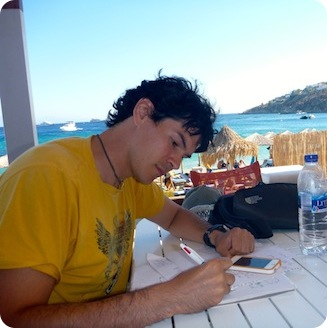
\includegraphics[width=.3\textwidth]{luis-b}% 
\hspace{.05\textwidth}%

\includegraphics[width=.3\textwidth]{rolf-b}% 
\hspace{.05\textwidth}%
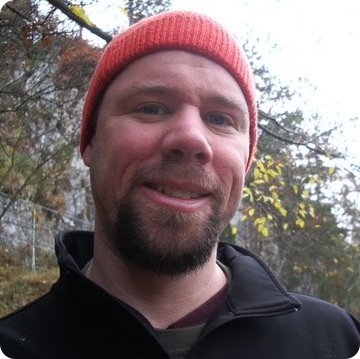
\includegraphics[width=.3\textwidth]{pat-b}%

\noindent\emph{Luis Barba.}
D\'epartement D'Informatique, Universit\'e Libre de Bruxelles
and
School of Computer Science, Carleton University

\noindent\emph{Rolf Fagerberg.}
Department of Mathematics and Computer Science, University of Southern Denmark

\noindent\emph{Pat Morin.}
School of Computer Scence, Carleton University

\end{document}


